\section{Investigating eBPF Performance Bottlenecks}
\label{sec:characterization}

A program compiled through the eBPF pipeline can run more slowly than native code compiled directly from the same source. This section quantifies the difference, investigates its sources, and discusses approaches to improving performance and the requirements they must meet.

\noindent\textbf{Microbenchmarks.}
We use 27 computational microbenchmarks to examine how compilation paths affect execution time. The benchmarks include simplified application logic and programs constructed around specific computations. For example, the Katran~\cite{katran} benchmark retains packet hashing and destination selection. Table~\ref{tab:microbenchmarks} lists their main computations. Their computation bodies make no helper calls or map accesses, reducing the influence of kernel services. All paths use the same computation source and fixed inputs.

\begin{table*}[t]
\centering
\small
\caption{Computational microbenchmarks used in Figure~\ref{fig:char-pure-percase}. The \texttt{cksum} and \texttt{tc\_cksum} programs perform the same computation with different eBPF program types.}
\label{tab:microbenchmarks}
\renewcommand{\arraystretch}{1.08}
\begin{tabular*}{\textwidth}{@{\extracolsep{\fill}}ll@{\hspace{1.2em}}ll@{\hspace{1.2em}}ll@{}}
\toprule
\textbf{Benchmark} & \textbf{Computation} & \textbf{Benchmark} & \textbf{Computation} & \textbf{Benchmark} & \textbf{Computation} \\
\midrule
\texttt{bitmap} & Bit counting, mixing & \texttt{katran} & Hash-based selection & \texttt{sock\_lb} & Service selection \\
\texttt{rule\_scan} & First-match scan & \texttt{policy} & Nested conditions & \texttt{tcpconn} & Connection filtering \\
\texttt{runqlat} & Logarithmic buckets & \texttt{siphash} & SipHash-style mixing & \texttt{tetragon} & Process-event filtering \\
\texttt{trace\_sw} & Switch dispatch & \texttt{bounds} & Bounds checks, reads & \texttt{otel} & Frame-record scan \\
\texttt{cksum} & Checksum & \texttt{field} & Field reads, mixing & \texttt{ct\_nat} & Address rewriting \\
\texttt{memcmp} & Bytewise comparison & \texttt{bitfield} & Bit-field extraction & \texttt{toeplitz} & Toeplitz-style hashing \\
\texttt{vlan} & Packet-header parsing & \texttt{str\_search} & Substring search & \texttt{fnv} & FNV-1a hashing \\
\texttt{call\_fanout} & Local-call dispatch & \texttt{syscall\_lookup} & Syscall label lookup & \texttt{tc\_cksum} & Checksum (TC) \\
\texttt{5tuple} & Jenkins-style hashing & \texttt{http} & HTTP prefix detection & \texttt{cgroup} & Hash mixing \\
\bottomrule
\end{tabular*}
\end{table*}


\noindent\textbf{Experimental setup.}
We use EC2 c7i.large instances for x86-64 and c7g.large instances for ARM64. The experiments use Clang 18.1.3 and a research kernel based on Linux 7.0.0-rc2. For each path, we take repeated measurements after warmup on 12 independent instances and compare mean execution time per invocation, excluding loading and compilation.

\subsection{Quantifying eBPF Slowdown}
\label{subsec:char-slowdown}

We compare execution time between the eBPF JIT and user-space native paths, using the same source and \texttt{-O2} for both. The eBPF path produces bytecode, which the kernel verifies and JIT-compiles before repeated execution through \texttt{BPF\_PROG\_TEST\_RUN}. The user-space native path compiles directly to native code and repeatedly invokes it through a function pointer.

\begin{figure*}[t]
\centering
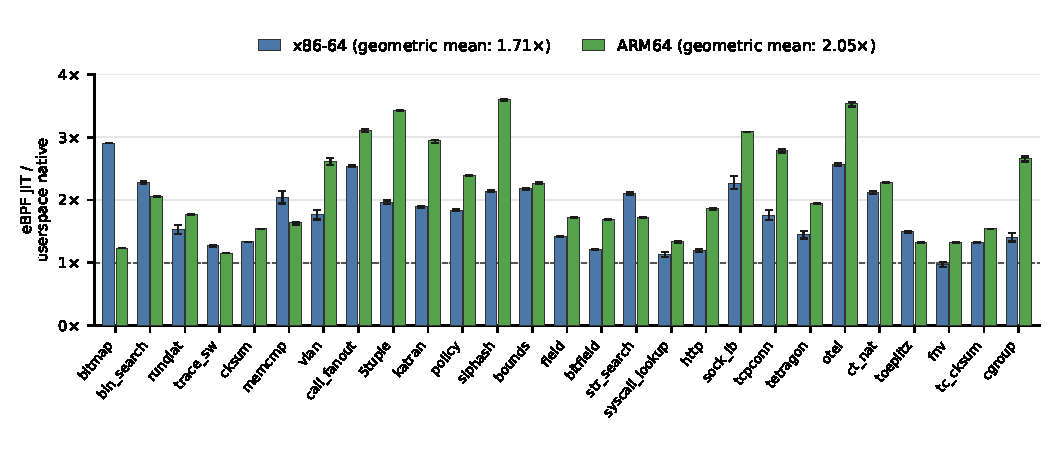
\includegraphics[width=\textwidth]{figures/sec-3-slowdown-o2-grouped.pdf}
\caption{eBPF JIT execution time relative to user-space native. The left and right bars for each benchmark correspond to x86-64 and ARM64. Each bar is the ratio of mean per-call execution times on the same architecture; values above 1 indicate slower eBPF JIT execution, and the dashed line denotes equal time. Error bars show 95\% confidence intervals obtained by resampling instances. Each geometric mean in the legend summarizes the 27 benchmark ratios for that architecture.}
\Description{Grouped bars compare eBPF JIT with user-space native across 27 benchmarks. Blue bars represent x86-64 and green bars represent ARM64, with geometric mean execution-time ratios of 1.71 and 2.05, respectively.}
\label{fig:char-pure-percase}
\end{figure*}


Figure~\ref{fig:char-pure-percase} shows that, across these benchmarks, programs generally run more slowly through the eBPF path than when compiled directly to native code from the same source. The geometric mean execution-time ratios are 1.71 on x86-64 and 2.05 on ARM64. For FNV on x86-64, the two paths have similar execution times. Machine-code comparisons show that both retain the byte-by-byte hash recurrence of exclusive OR and multiplication; direct native compilation does not shorten this dependency chain.

\subsection{Investigating Sources of eBPF Slowdown}
\label{subsec:char-sources}
\label{subsec:char-idiom}

To investigate why eBPF programs run more slowly than user-space native programs compiled from the same source, we first examine whether the difference in execution location explains the slowdown. We run the user-space native compilation output in the kernel through the same test-run interface as the eBPF JIT. Both native paths use only general-purpose registers, so kernel execution requires no additional saving and restoring of floating-point or SIMD registers~\cite{linuxndfloatingpoint}.

Table~\ref{tab:char-micro-summary} shows that the performance advantage of direct native compilation persists in the kernel. Although kernel native execution takes about 6\% longer than user-space native execution on x86-64 and 15\% longer on ARM64 overall, it remains faster than JIT-compiled eBPF code running in the same kernel.

\begin{finding}[unbreakable]
\finlabel Execution location does not fully explain the performance difference between the eBPF JIT and direct native compilation. With both running in the kernel, JIT-compiled eBPF code still takes 1.62$\times$ as long as native code on x86-64 and 1.77$\times$ on ARM64 overall.
\end{finding}

We next examine whether limitations of eBPF bytecode itself account for the performance difference between the eBPF JIT and direct native compilation. We compare native code regenerated from eBPF bytecode with directly compiled native code, running both in user space. LLVM-BPF~\cite{zheng2025extending} is an LLVM-based user-space eBPF compiler that translates bytecode into LLVM IR, optimizes it, and generates native code. We give LLVM-BPF the same bytecode as the eBPF JIT, use O2 optimization, and select the same target CPU and instruction features as direct native compilation. Table~\ref{tab:char-micro-summary} shows that LLVM-BPF approaches the overall performance of direct native compilation, demonstrating that these programs can still have efficient implementations after passing through eBPF bytecode.

\begin{table}[t]
\centering
\small
\caption{Execution-time ratios on x86-64 and ARM64. Each entry is the geometric mean of the 27 ratios of mean per-call execution times, with the numerator and denominator given in the first column. Values above 1 indicate a slower numerator path.}
\label{tab:char-micro-summary}
\begin{tabular}{@{}lcc@{}}
\toprule
\textbf{Execution-time ratio} & \textbf{x86-64} & \textbf{ARM64} \\
\midrule
Kernel native / user-space native & 1.055 & 1.154 \\
\addlinespace
eBPF JIT / kernel native & 1.622 & 1.773 \\
\addlinespace
LLVM-BPF / user-space native & 1.068 & 1.054 \\
\bottomrule
\end{tabular}
\end{table}


\begin{finding}[unbreakable]
\finlabel Using eBPF bytecode does not prevent these programs from approaching the overall performance of direct native compilation. In user space, code generated by LLVM-BPF takes about 7\% longer than native code on x86-64 and 5\% longer on ARM64 overall.
\end{finding}

We further analyze why the eBPF compilation pipeline does not fully exploit the target CPU's instructions. LLVM's BPF back end optimizes and selects instructions for the eBPF instruction set, whereas direct native compilation targets the final CPU~\cite{llvmndcodegenerator}. Some computations that a single native instruction can perform therefore require multiple basic operations in bytecode. eBPF is designed to make it easy for a JIT to map basic instructions to native architectures~\cite{linuxndclassicbpf}. Selecting a native instruction for the full computation requires recognizing how its basic operations relate.

The rotation in Figure~\ref{fig:jit-dump} illustrates this process. eBPF has no rotate instruction~\cite{rfc9669}, so LLVM's BPF back end expands rotations into basic operations~\cite{llvmndbpflowering}. A 64-bit left rotation by 16 bits in the SipHash-style microbenchmark consists of a copy, two shifts, and a bitwise OR. The current x86-64 JIT emits \texttt{MOV; SHR; SHL; OR}, whereas direct native compilation emits a single \texttt{RORX}. The bytecode fully preserves the rotation computation, but expresses it across several instructions. The current JIT selects native implementations from each instruction's opcode and operands, retaining this sequence because it does not analyze their data dependencies to recognize rotation.

\begin{figure}[t]
\centering
\begin{tikzpicture}[
  x=1cm,y=1cm,
  font=\sffamily\fontsize{8}{9.5}\selectfont,
  code/.style={draw=black,line width=0.5pt,fill=black!2,
    text width=3.1cm,inner xsep=2mm,inner ysep=2mm,
    anchor=north west,align=left,
    font=\ttfamily\fontsize{8}{9.5}\selectfont},
  heading/.style={anchor=south west,text depth=1.5pt,font=\sffamily\bfseries\fontsize{8}{9.5}\selectfont},
  flow/.style={-{Stealth[length=1.5mm]},line width=0.6pt},
  stage/.style={align=center,font=\sffamily\fontsize{7.5}{9}\selectfont}
]
\path[use as bounding box] (0,-0.08) rectangle (8.5,4.72);
\node[heading] at (0,4.21) {C (simplified)};
\node[heading] at (5,4.21) {x86-64 native};
\node[code,minimum height=1.35cm] (source) at (0,4.15) {y = (x <{}< 16)\\\hspace*{1em}| (x >{}> 48);};
\node[code,minimum height=1.35cm] (native) at (5,4.15) {rorx r15, rbx, 0x30};
\node[heading,align=left] at (0,1.76) {eBPF\\bytecode};
\node[heading] at (5,1.76) {x86-64 native};
\node[code,minimum height=1.75cm] (bytecode) at (0,1.70) {r1 = r7\\r1 >{}>= 48\\r7 <{}<= 16\\r7 |= r1};
\node[code,minimum height=1.75cm] (jit) at (5,1.70) {mov rdi, r13\\shr rdi, 0x30\\shl r13, 0x10\\or r13, rdi};
\draw[flow] (source.east) -- node[above,stage] {Clang\\(native)} (native.west);
\draw[flow] (source.south) -- node[right,stage] {Clang (BPF)} (bytecode.north);
\draw[flow] (bytecode.east) -- node[above,stage] {eBPF JIT} (jit.west);
\end{tikzpicture}
\caption{Two compilation paths for a 64-bit left rotation by 16 bits in the SipHash-style benchmark on x86-64. In the simplified C expression, \texttt{x} and \texttt{y} are 64-bit unsigned integers. The code panels show only the rotation, omitting input preparation and adjacent computation. Assembly uses Intel syntax; right rotation by \texttt{0x30} (48) bits equals left rotation by 16 bits.}
\Description{A two-by-two diagram compares direct native compilation with compilation through eBPF. Simplified C for the constant-16 rotation produces one RORX instruction through direct compilation, or a register copy, two shifts, and an OR through eBPF and its JIT.}
\label{fig:jit-dump}
\end{figure}


Table~\ref{tab:isa-gap} compares the generated code for bit extraction and big-endian reads, which also offer opportunities to combine basic operations or memory accesses. The halfword load and byte-order conversion needed for the big-endian read already exist in the eBPF instruction set. These opportunities extend beyond computations without a dedicated eBPF instruction.

\begin{table*}[t]
\centering
\small
\caption{Native instruction sequences for two computations in the compiled programs. The operand \texttt{b} is a zero-extended byte. Bit extraction starts with the operand ready; the big-endian read includes the memory loads.}
\label{tab:isa-gap}
\begin{tabular}{@{}llll@{}}
\toprule
\textbf{Computation} & \textbf{Architecture} & \textbf{eBPF JIT} & \textbf{Direct native} \\
\midrule
\texttt{(b >{}> 1) \& 0x1f} & ARM64 & \texttt{LSR; AND} & \texttt{UBFX} \\
Big-endian 16-bit read & x86-64 & \texttt{MOVZX} $\times$ 2\texttt{; SHL; OR; AND} & \texttt{MOVBE; MOVZX} \\
Big-endian 16-bit read & ARM64 & \texttt{LDRB} $\times$ 2\texttt{; LSL; ORR; AND} & \texttt{LDRH; REV16} \\
\bottomrule
\end{tabular}
\end{table*}


\begin{finding}[unbreakable]
\finlabel The current eBPF compilation pipeline misses some opportunities to combine operations for the target CPU. User-space compilation produces combinations of basic eBPF operations, while the subsequent JIT mainly maps individual instructions without recognizing the combinations that enable more compact native code.
\end{finding}

\subsection{Design Implications}
\label{subsec:char-challenges}

The code comparisons show that some combinations of operations admit more compact native implementations. Taking advantage of these opportunities requires recognizing these combinations in a program and selecting their implementations for the target architecture.

Existing approaches have limitations in supporting these native optimizations. K2~\cite{xu2021synthesizing}, Merlin~\cite{mao2024merlin}, and EPSO~\cite{zhu2025epso} rewrite programs in user space, combining operations and eliminating redundancy using existing eBPF instructions, then pass the results to the existing verifier and JIT. These methods can improve generated code, but rewriting ordinary bytecode alone cannot select a native implementation for which the JIT has no selection rule. Enhancing the JIT directly can add such rules, but requires adding the corresponding pattern analysis, transformation checks, and code generation to the kernel. As the set of optimizations grows, so does the kernel code that must be maintained and reviewed. In addition, these transformations occur after verification: incorrect matching or code generation can change program behavior and invalidate the safety guarantee established by the verifier. Shahinfar et al.~\cite{shahinfar2026fun} propose generating native code directly with a user-space optimizer after verification. This keeps the optimization implementation outside the kernel, but safe execution still requires a trusted translation process or additional checks on the generated code.

We investigate how to integrate local native operations while limiting the size and complexity of the trusted code added to the kernel. Extensions must preserve observable program behavior across optimization and ensure that the verifier's safety conclusions apply to the machine code that executes. New operations should then reuse the integration and verification mechanisms and support native implementations of the same operation across architectures, reducing extension and maintenance costs. Section~\ref{sec:mechanism} describes the design of \tool.
